\documentclass[tikz,border=3.14mm]{standalone}
\begin{document}
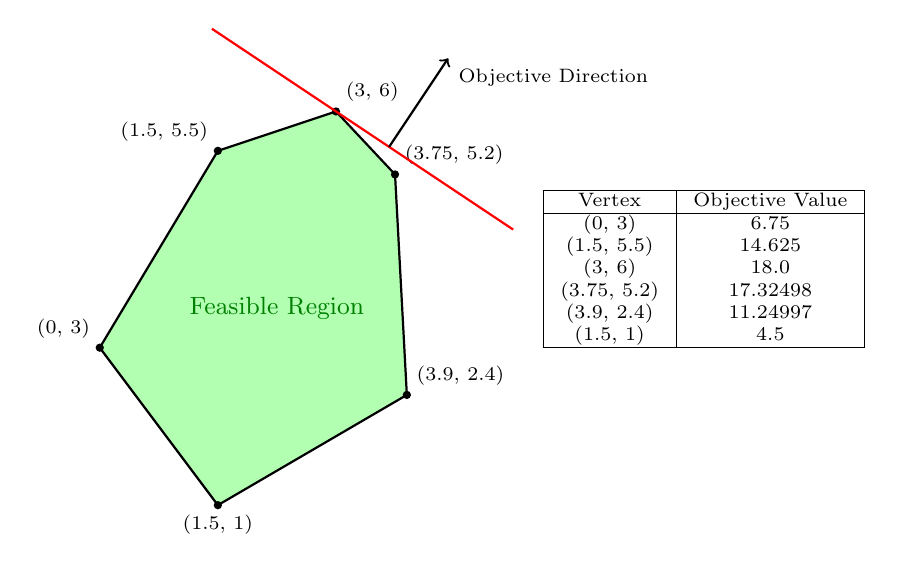
\begin{tikzpicture}

    % Define direction d as a variable
    \pgfmathsetmacro{\dx}{2.25} % Adjusted for 1.5x scaling
    \pgfmathsetmacro{\dy}{-1.5}

    % Compute perpendicular direction to d
    \pgfmathsetmacro{\dperpx}{-\dy}
    \pgfmathsetmacro{\dperpy}{\dx}

    % Define vertices
    \pgfmathsetmacro{\xA}{0}
    \pgfmathsetmacro{\yA}{3}
    \pgfmathsetmacro{\xB}{1.5}
    \pgfmathsetmacro{\yB}{5.5}
    \pgfmathsetmacro{\xC}{3}
    \pgfmathsetmacro{\yC}{6}
    \pgfmathsetmacro{\xD}{3.75}
    \pgfmathsetmacro{\yD}{5.2}
    \pgfmathsetmacro{\xE}{3.9}
    \pgfmathsetmacro{\yE}{2.4}
    \pgfmathsetmacro{\xF}{1.5}
    \pgfmathsetmacro{\yF}{1}

    % Compute objective values
    \pgfmathsetmacro{\objA}{\xA*\dperpx + \yA*\dperpy}
    \pgfmathsetmacro{\objB}{\xB*\dperpx + \yB*\dperpy}
    \pgfmathsetmacro{\objC}{\xC*\dperpx + \yC*\dperpy}
    \pgfmathsetmacro{\objD}{\xD*\dperpx + \yD*\dperpy}
    \pgfmathsetmacro{\objE}{\xE*\dperpx + \yE*\dperpy}
    \pgfmathsetmacro{\objF}{\xF*\dperpx + \yF*\dperpy}

    % Define the polygon fill
    \fill[green!30] 
        (\xA,\yA) -- (\xB,\yB) -- (\xC,\yC) -- (\xD,\yD) -- (\xE,\yE) -- (\xF,\yF) -- cycle;

    % Draw the polygon outline
    \draw[thick] 
        (\xA,\yA) -- (\xB,\yB) -- (\xC,\yC) -- (\xD,\yD) -- (\xE,\yE) -- (\xF,\yF) -- cycle;

    % Draw the nodes (points) and label them with coordinates
    \foreach \x/\y in {3/6, 3.75/5.2, 3.9/2.4} {
        \fill[black] (\x,\y) circle (1.5pt);
        \node[font=\scriptsize, above right] at (\x,\y) {(\x, \y)};
    }
    \foreach \x/\y in {0/3, 1.5/5.5} {
        \fill[black] (\x,\y) circle (1.5pt);
        \node[font=\scriptsize, above left] at (\x,\y) {(\x, \y)};
    }
    \foreach \x/\y in {1.5/1} {
        \fill[black] (\x,\y) circle (1.5pt);
        \node[font=\scriptsize, below] at (\x,\y) {(\x, \y)};
    }

    % Define the red line through (3,6) in direction d
    \draw[red, thick] 
        ({\xC + \dx}, {\yC + \dy}) -- ({\xC - 0.7*\dx}, {\yC - 0.7*\dy});

    % Add a perpendicular arrow at (3,6)
    \draw[->, thick] 
        ({\xC + 0.3*\dx}, {\yC + 0.3*\dy}) -- 
        ({\xC + 0.3*\dx + 0.5*\dperpx}, {\yC + 0.3*\dy + 0.5*\dperpy})
        node[below right, font=\scriptsize] {Objective Direction};

    % Add a label for the feasible region
    \node[green!50!black, font=\small] at (2.25, 3.5) {Feasible Region};

    % Add an arrow pointing to a vertex and label the vertex
%    \draw[->, thick, blue] (4.5, 2.4) -- (3.9,2.4) 
%        node[midway, above right, black, font=\scriptsize] {Vertex};

    % Add a table of objective values on the right
    \node[anchor=west, font=\scriptsize] at (5.5, 4) {
        \begin{tabular}{|c|c|}
        \hline
        Vertex & Objective Value \\
        \hline
        (\xA, \yA) & \objA \\
        (\xB, \yB) & \objB \\
        (\xC, \yC) & \objC \\
        (\xD, \yD) & \objD \\
        (\xE, \yE) & \objE \\
        (\xF, \yF) & \objF \\
        \hline
        \end{tabular}
    };

\end{tikzpicture}
\end{document}
